%%%%%%%%%%%%%%%%%%%%%%%%%%%%%%%%%%%%%%%%%%%%%%%%%%%
%% LaTeX book template                           %%
%% Author:  Amber Jain (http://amberj.devio.us/) %%
%% License: ISC license                          %%
%%%%%%%%%%%%%%%%%%%%%%%%%%%%%%%%%%%%%%%%%%%%%%%%%%%

\documentclass[a4paper,12pt]{book}
\usepackage[T1]{fontenc}
\usepackage[utf8]{inputenc}
\usepackage{lmodern}
%%%%%%%%%%%%%%%%%%%%%%%%%%%%%%%%%%%%%%%%%%%%%%%%%%%%%%%%%
% Source: http://en.wikibooks.org/wiki/LaTeX/Hyperlinks %
%%%%%%%%%%%%%%%%%%%%%%%%%%%%%%%%%%%%%%%%%%%%%%%%%%%%%%%%%
\usepackage{hyperref}
\usepackage{graphicx}
\usepackage[english]{babel}
\usepackage{CTEX}
% \usepackage{hyperref}
% % 格式设置
% \hypersetup{hidelinks,
% 	colorlinks=true,
% 	allcolors=pink,
% 	pdfstartview=Fit,
% 	breaklinks=true
% }


%%%%%%%%%%%%%%%%%%%%%%%%%%%%%%%%%%%%%%%%%%%%%%%%%%%%%%%%%%%%%%%%%%%%%%%%%%%%%%%%
% 'dedication' environment: To add a dedication paragraph at the start of book %
% Source: http://www.tug.org/pipermail/texhax/2010-June/015184.html            %
%%%%%%%%%%%%%%%%%%%%%%%%%%%%%%%%%%%%%%%%%%%%%%%%%%%%%%%%%%%%%%%%%%%%%%%%%%%%%%%%
\newenvironment{dedication}
{
   \cleardoublepage
   \thispagestyle{empty}
   \vspace*{\stretch{1}}
   \hfill\begin{minipage}[t]{0.66\textwidth}
   \raggedright
}
{
   \end{minipage}
   \vspace*{\stretch{3}}
   \clearpage
}

%%%%%%%%%%%%%%%%%%%%%%%%%%%%%%%%%%%%%%%%%%%%%%%%
% Chapter quote at the start of chapter        %
% Source: http://tex.stackexchange.com/a/53380 %
%%%%%%%%%%%%%%%%%%%%%%%%%%%%%%%%%%%%%%%%%%%%%%%%
\makeatletter
\renewcommand{\@chapapp}{}% Not necessary...
\newenvironment{chapquote}[2][2em]
  {\setlength{\@tempdima}{#1}%
   \def\chapquote@author{#2}%
   \parshape 1 \@tempdima \dimexpr\textwidth-2\@tempdima\relax%
   \itshape}
  {\par\normalfont\hfill--\ \chapquote@author\hspace*{\@tempdima}\par\bigskip}
\makeatother

%%%%%%%%%%%%%%%%%%%%%%%%%%%%%%%%%%%%%%%%%%%%%%%%%%%
% First page of book which contains 'stuff' like: %
%  - Book title, subtitle                         %
%  - Book author name                             %
%%%%%%%%%%%%%%%%%%%%%%%%%%%%%%%%%%%%%%%%%%%%%%%%%%%

% Book's title and subtitle
\title{
  \Huge \textbf{Anolang设计手册}  
  \footnote{名字源于Mygo传奇吉他手Anon Chihaya.} \\ 
  \huge 一门独属于邦邦人的编程语言. 
  \footnote{写给自己的,纯属娱乐性质的一门语言}
}

% Author
\author{
  \textsc{Zhuiri Xiao}
  \thanks{\url{https://github.com/paitsai/anolang.git}}
}


\begin{document}

\frontmatter
\maketitle
%%%%%%%%%%%%%%%%%%%%%%%%%%%%%%%%%%%%%%%%%%%%%%%%%%%%%%%%%%%%%%%
% Add a dedication paragraph to dedicate your book to someone %
%%%%%%%%%%%%%%%%%%%%%%%%%%%%%%%%%%%%%%%%%%%%%%%%%%%%%%%%%%%%%%%
\begin{dedication}
  “\\ \quad 僅僅遭遇過一次失敗卻不懂得重新開始,人生這麼長會撐不住的哦。\\”\\
  \qquad Anon Chihaya \\ \quad @ \today

\end{dedication}

%%%%%%%%%%%%%%%%%%%%%%%%%%%%%%%%%%%%%%%%%%%%%%%%%%%%%%%%%%%%%%%%%%%%%%%%
% Auto-generated table of contents, list of figures and list of tables %
%%%%%%%%%%%%%%%%%%%%%%%%%%%%%%%%%%%%%%%%%%%%%%%%%%%%%%%%%%%%%%%%%%%%%%%%
\tableofcontents
% \listoffigures
% \listoftables

\mainmatter

%%%%%%%%%%%
% Preface %
%%%%%%%%%%%
\chapter{Preface}



這是本人\footnote{\url{https://github.com/paitsai}}開始於2024.12的設計的Anolang編譯器\footnote{\url{https://github.com/paitsai/anolang}},不知道需要歷時多久?希望能夠在畢業之前完成這個項目。
和普遍的編譯器一樣,Anolang的編譯器同樣采用前端+優化器+後端的三級架構。

% Lorem ipsum dolor sit amet, consectetur adipiscing elit. Duis risus ante, auctor et pulvinar non, posuere ac lacus. Praesent egestas nisi id metus rhoncus ac lobortis sem hendrerit. Etiam et sapien eget lectus interdum posuere sit amet ac urna.

% \section*{Un-numbered sample section}
% Lorem ipsum dolor sit amet, consectetur adipiscing elit. Duis risus ante, auctor et pulvinar non, posuere ac lacus. Praesent egestas nisi id metus rhoncus ac lobortis sem hendrerit. Etiam et sapien eget lectus interdum posuere sit amet ac urna. Aliquam pellentesque imperdiet erat, eget consectetur felis malesuada quis. Pellentesque sollicitudin, odio sed dapibus eleifend, magna sem luctus turpis.

% \section*{Another sample section}
% Lorem ipsum dolor sit amet, consectetur adipiscing elit. Duis risus ante, auctor et pulvinar non, posuere ac lacus. Praesent egestas nisi id metus rhoncus ac lobortis sem hendrerit. Etiam et sapien eget lectus interdum posuere sit amet ac urna. Aliquam pellentesque imperdiet erat, eget consectetur felis malesuada quis. Pellentesque sollicitudin, odio sed dapibus eleifend, magna sem luctus turpis, id aliquam felis dolor eu diam. Etiam ullamcorper, nunc a accumsan adipiscing, turpis odio bibendum erat, id convallis magna eros nec metus.

% \section*{Structure of book}
% % You might want to add short description about each chapter in this book.
% Each unit will focus on <SOMETHING>.

% \section*{About the companion website}
% The website\footnote{\url{https://github.com/amberj/latex-book-template}} for this file contains:
% \begin{itemize}
%   \item A link to (freely downlodable) latest version of this document.
%   \item Link to download LaTeX source for this document.
%   \item Miscellaneous material (e.g. suggested readings etc).
% \end{itemize}

% %%%%%%%%%%%%%%%%%%%%%%%%%%%%%%%%%%%%
% % Give credit where credit is due. %
% % Say thanks!                      %
% %%%%%%%%%%%%%%%%%%%%%%%%%%%%%%%%%%%%
% \section*{Acknowledgements}
% \begin{itemize}
% \item A special word of thanks goes to Professor Don Knuth\footnote{\url{http://www-cs-faculty.stanford.edu/~uno/}} (for \TeX{}) and Leslie Lamport\footnote{\url{http://www.lamport.org/}} (for \LaTeX{}).
% \item I'll also like to thank Gummi\footnote{\url{http://gummi.midnightcoding.org/}} developers and LaTeXila\footnote{\url{http://projects.gnome.org/latexila/}} development team for their awesome \LaTeX{} editors.
% \item I'm deeply indebted my parents, colleagues and friends for their support and encouragement.
% \end{itemize}
% \mbox{}\\
% %\mbox{}\\
% \noindent Amber Jain \\
% \noindent \url{http://amberj.devio.us/}

%%%%%%%%%%%%%%%%
% NEW CHAPTER! %
%%%%%%%%%%%%%%%%



\chapter{編譯器前端}
傳統意義上,編譯器前端需要完成什麼任務?
编译器的“前端”指的是编译器对程序代码的分析和理解过程。

\begin{figure}[htbp]
    \centering
    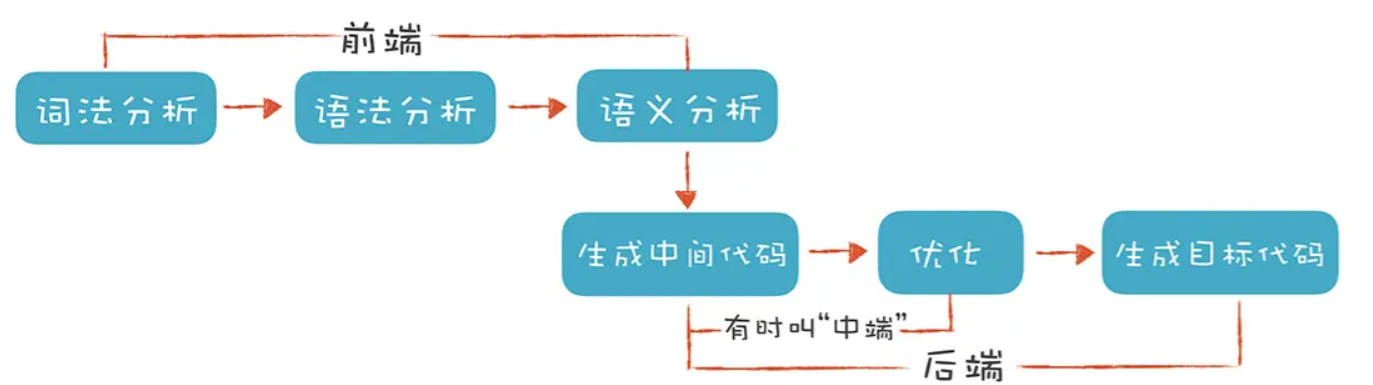
\includegraphics[scale=0.4]{pics/font1.png}
    \caption{編譯器架構}
    \label{p}
\end{figure}
    

编译器的“前端”技术分为词法分析、语法分析和
语义分析三个部分。
而它主要涉及自动机和形式语言方面的基础的计算理论。


\section{詞法分析}

詞法分析是將程式碼轉換為一個個的詞彙項目(Token)的過程。
像一段代碼中我们会识别出 if、else、int 这样的关键字,
main、printf、age 这样的标识符,+、-、= 这样的操作符号,
还有花括号、圆括号、分号这样的符号,以及数字字面量、字符串字面量等。
这些都是 Token。


\end{document}
